\documentclass[11pt]{article}
\usepackage[margin=0.92in]{geometry}
\usepackage{lmodern}
\usepackage[T1]{fontenc}
\usepackage{amsmath,amssymb,amsthm}
\usepackage{booktabs,tabularx}
\usepackage{graphicx,microtype}
\usepackage[dvipsnames]{xcolor}
\usepackage[numbers,sort&compress]{natbib}
\usepackage[colorlinks=true,linkcolor=MidnightBlue,citecolor=MidnightBlue,urlcolor=MidnightBlue]{hyperref}
\usepackage{caption,placeins,needspace}
\hypersetup{pdftitle={When Does Forecast-Aware Sensor Placement Help?},pdfauthor={A. S. M. Jahir Hossain},pdfsubject={A reproducible stress test of shifting line traffic}}
\usepackage{fancyhdr}
\pagestyle{fancy}
\fancyhf{}
\fancyhead[L]{\small\textsf{STOCHPLACE / RESEARCH SOFTWARE STUDY}}
\fancyhead[R]{\small\textsf{REVISION 2.1}}
\fancyfoot[C]{\small\thepage}
\setlength{\headheight}{14pt}
\setlength{\parskip}{4pt}
\renewcommand{\topfraction}{0.95}
\renewcommand{\textfraction}{0.04}
\renewcommand{\floatpagefraction}{0.9}
\newtheorem{proposition}{Proposition}
\newcommand{\E}{\mathbb E}
\newcommand{\R}{\mathbb R}
\graphicspath{{../docs/figures/}}
% generated by scripts/make_tables.py from results/; do not edit
\newcommand{\missRedStat}{0.5}
\newcommand{\missRedLoStat}{-0.2}
\newcommand{\missRedHiStat}{1.5}
\newcommand{\gapClosedStat}{7}
\newcommand{\mixClosedStat}{-17}
\newcommand{\histMissStat}{3.42}
\newcommand{\stackMissStat}{3.41}
\newcommand{\oracleMissStat}{3.18}
\newcommand{\winRateStat}{30}
\newcommand{\missRedDrift}{37.6}
\newcommand{\missRedLoDrift}{36.1}
\newcommand{\missRedHiDrift}{39.1}
\newcommand{\gapClosedDrift}{93}
\newcommand{\mixClosedDrift}{72}
\newcommand{\histMissDrift}{7.41}
\newcommand{\stackMissDrift}{4.62}
\newcommand{\oracleMissDrift}{4.43}
\newcommand{\winRateDrift}{100}
\newcommand{\missRedShift}{36.3}
\newcommand{\missRedLoShift}{34.7}
\newcommand{\missRedHiShift}{37.8}
\newcommand{\gapClosedShift}{83}
\newcommand{\mixClosedShift}{-5}
\newcommand{\histMissShift}{3.20}
\newcommand{\stackMissShift}{2.04}
\newcommand{\oracleMissShift}{1.81}
\newcommand{\winRateShift}{100}
\newcommand{\missRedEmerg}{32.8}
\newcommand{\missRedLoEmerg}{24.8}
\newcommand{\missRedHiEmerg}{39.2}
\newcommand{\gapClosedEmerg}{85}
\newcommand{\mixClosedEmerg}{-23}
\newcommand{\histMissEmerg}{5.15}
\newcommand{\stackMissEmerg}{3.46}
\newcommand{\oracleMissEmerg}{3.17}
\newcommand{\winRateEmerg}{95}
\newcommand{\apxN}{100}
\newcommand{\apxMin}{0.9470}
\newcommand{\apxOpt}{25}
\newcommand{\apxRefine}{100}
\newcommand{\boundRuns}{7{,}360}
\newcommand{\boundHoldsA}{100.0}
\newcommand{\boundHoldsB}{100.0}
\newcommand{\boundRhoA}{0.82}
\newcommand{\boundRhoB}{0.80}
\newcommand{\sweepHistHone}{2.2}
\newcommand{\sweepHistHthree}{4.2}
\newcommand{\sweepStackMax}{0.23}
\newcommand{\sweepTrendHthree}{13.9}
\newcommand{\sweepRecentHthree}{10.4}
\newcommand{\voidGainDUStat}{0.16}
\newcommand{\voidGainDULoStat}{0.11}
\newcommand{\voidGainDUHiStat}{0.21}
\newcommand{\voidGainSTStat}{-0.02}
\newcommand{\voidGainSTLoStat}{-0.05}
\newcommand{\voidGainSTHiStat}{0.01}
\newcommand{\wPooledStat}{0.87}
\newcommand{\wRecentStat}{0.12}
\newcommand{\wDriftuStat}{0.01}
\newcommand{\wTrendStat}{0.00}
\newcommand{\voidGainDUDrift}{0.00}
\newcommand{\voidGainDULoDrift}{-0.01}
\newcommand{\voidGainDUHiDrift}{0.01}
\newcommand{\voidGainSTDrift}{-3.47}
\newcommand{\voidGainSTLoDrift}{-4.24}
\newcommand{\voidGainSTHiDrift}{-2.70}
\newcommand{\wPooledDrift}{0.00}
\newcommand{\wRecentDrift}{0.00}
\newcommand{\wDriftuDrift}{0.87}
\newcommand{\wTrendDrift}{0.12}
\newcommand{\voidGainDUShift}{0.08}
\newcommand{\voidGainDULoShift}{-0.08}
\newcommand{\voidGainDUHiShift}{0.20}
\newcommand{\voidGainSTShift}{-0.01}
\newcommand{\voidGainSTLoShift}{-0.05}
\newcommand{\voidGainSTHiShift}{0.04}
\newcommand{\wPooledShift}{0.00}
\newcommand{\wRecentShift}{0.19}
\newcommand{\wDriftuShift}{0.00}
\newcommand{\wTrendShift}{0.81}
\newcommand{\voidGainDUEmerg}{0.48}
\newcommand{\voidGainDULoEmerg}{0.28}
\newcommand{\voidGainDUHiEmerg}{0.70}
\newcommand{\voidGainSTEmerg}{-0.03}
\newcommand{\voidGainSTLoEmerg}{-0.19}
\newcommand{\voidGainSTHiEmerg}{0.17}
\newcommand{\wPooledEmerg}{0.27}
\newcommand{\wRecentEmerg}{0.29}
\newcommand{\wDriftuEmerg}{0.13}
\newcommand{\wTrendEmerg}{0.31}
\newcommand{\scarcePooled}{0.99}
\newcommand{\scarceLgcp}{3.25}
\newcommand{\scarceLgcpVoid}{1.93}
\newcommand{\scarceLgcpCvar}{6.79}
\newcommand{\aisPooled}{76.6}
\newcommand{\aisStacked}{77.7}
\newcommand{\aisHindsight}{85.0}
\newcommand{\aisFence}{63.8}
\newcommand{\aisRandom}{39.8}
\newcommand{\aisOrigins}{4}
\newcommand{\aisReports}{84{,}702}
\newcommand{\aisLines}{265}

% generated by scripts/research_summary.py; do not edit
\newcommand{\reversalHistory}{94.03}
\newcommand{\reversalStacked}{89.53}
\newcommand{\robustGridErrorMax}{0.18}
\newcommand{\tvPenaltyFiveMin}{4.93}
\newcommand{\tvPenaltyFiveMax}{5.00}
\newcommand{\tvPenaltyFifteenMin}{14.73}
\newcommand{\tvPenaltyFifteenMax}{14.99}
\newcommand{\tvSmallCoverageMax}{0}
\newcommand{\tvCoverageDrift}{95}
\newcommand{\tvCoverageEmergence}{0}
\newcommand{\tvCoverageLaneShift}{0}
\newcommand{\tvCoverageReversal}{0}
\newcommand{\tvCoverageSeamDrift}{95}
\newcommand{\tvCoverageStationary}{95}

% generated by scripts/void_failure_analysis.py; do not edit
\newcommand{\voidDriftGap}{3.67}
\newcommand{\voidDriftGapLo}{2.90}
\newcommand{\voidDriftGapHi}{4.44}
\newcommand{\voidDriftHistory}{-0.69}
\newcommand{\voidDriftHistoryLo}{-1.46}
\newcommand{\voidDriftHistoryHi}{0.11}
\newcommand{\voidDriftCorr}{0.70}
\newcommand{\voidDriftSeeds}{40}
\newcommand{\voidDriftOverOne}{29}

% generated by scripts/ais_bandwidth_sensitivity.py; do not edit
\newcommand{\aisBandwidthGapMin}{7.5}
\newcommand{\aisBandwidthGapMax}{8.6}
\newcommand{\aisFinePooled}{84.8}
\newcommand{\aisFineStacked}{85.0}
\newcommand{\aisFineLgcp}{85.2}
\newcommand{\aisFineRecentGap}{2.4}

% Generated by scripts/presentation_summary.py; do not edit.
\newcommand{\overviewAISHistory}{84.78}
\newcommand{\overviewAISStacked}{82.55}
\newcommand{\overviewComponentGap}{6.83}
\newcommand{\overviewWFailures}{6}
\newcommand{\overviewWRegimes}{6}

\title{\textbf{When Does Forecast-Aware\\Sensor Placement Help?}\\[5pt]
\large A reproducible stress test of shifting line traffic}
\author{A.\,S.\,M. Jahir Hossain\\[4pt]
\small Independent research software extension and comparative study\\
\small\url{https://github.com/Zahir-Hossain/stochastic-sensor-placement-extension}}
\date{Technical report / November 2026 / Version 2.1}

\begin{document}
\maketitle
\thispagestyle{empty}

\begin{abstract}
A fixed sensor network must detect traffic that may change after placement.
We compare chronological Poisson intensity stacking, historical planning,
individual forecasters, nonlinear risk objectives and ambiguity sets.
In three designed shifts that match a candidate, stacking reduces expected
misses by \missRedEmerg--\missRedDrift\% over history across 40 paired seeds.
It loses under an unannounced reversal. In five additional shift regimes,
it improves on pooled history but has lower mean detection than the best
single component, by up to \overviewComponentGap{} percentage points.
On one reused AIS day, training-selected historical KDE averages
\overviewAISHistory\% modelled detection versus \overviewAISStacked\% for
stacking over four overlapping origins; the bandwidth grid is exhausted
at its lower edge. TV ambiguity barely changes future detection, while
transport ambiguity lowers its mean in \overviewWFailures/\overviewWRegimes{}
regimes under the fixed radius-calibration rule. The current forecast
sampler and both alternatives fail the frozen diagnostic gate.
These results establish neither calibrated uncertainty nor operational
performance. The extension design was frozen locally before its outcomes,
without an external preregistration timestamp. Raw runs, numerical checks
and source fingerprints make both successes and failures reproducible.
\end{abstract}

\begin{figure}[!htbp]
\centering
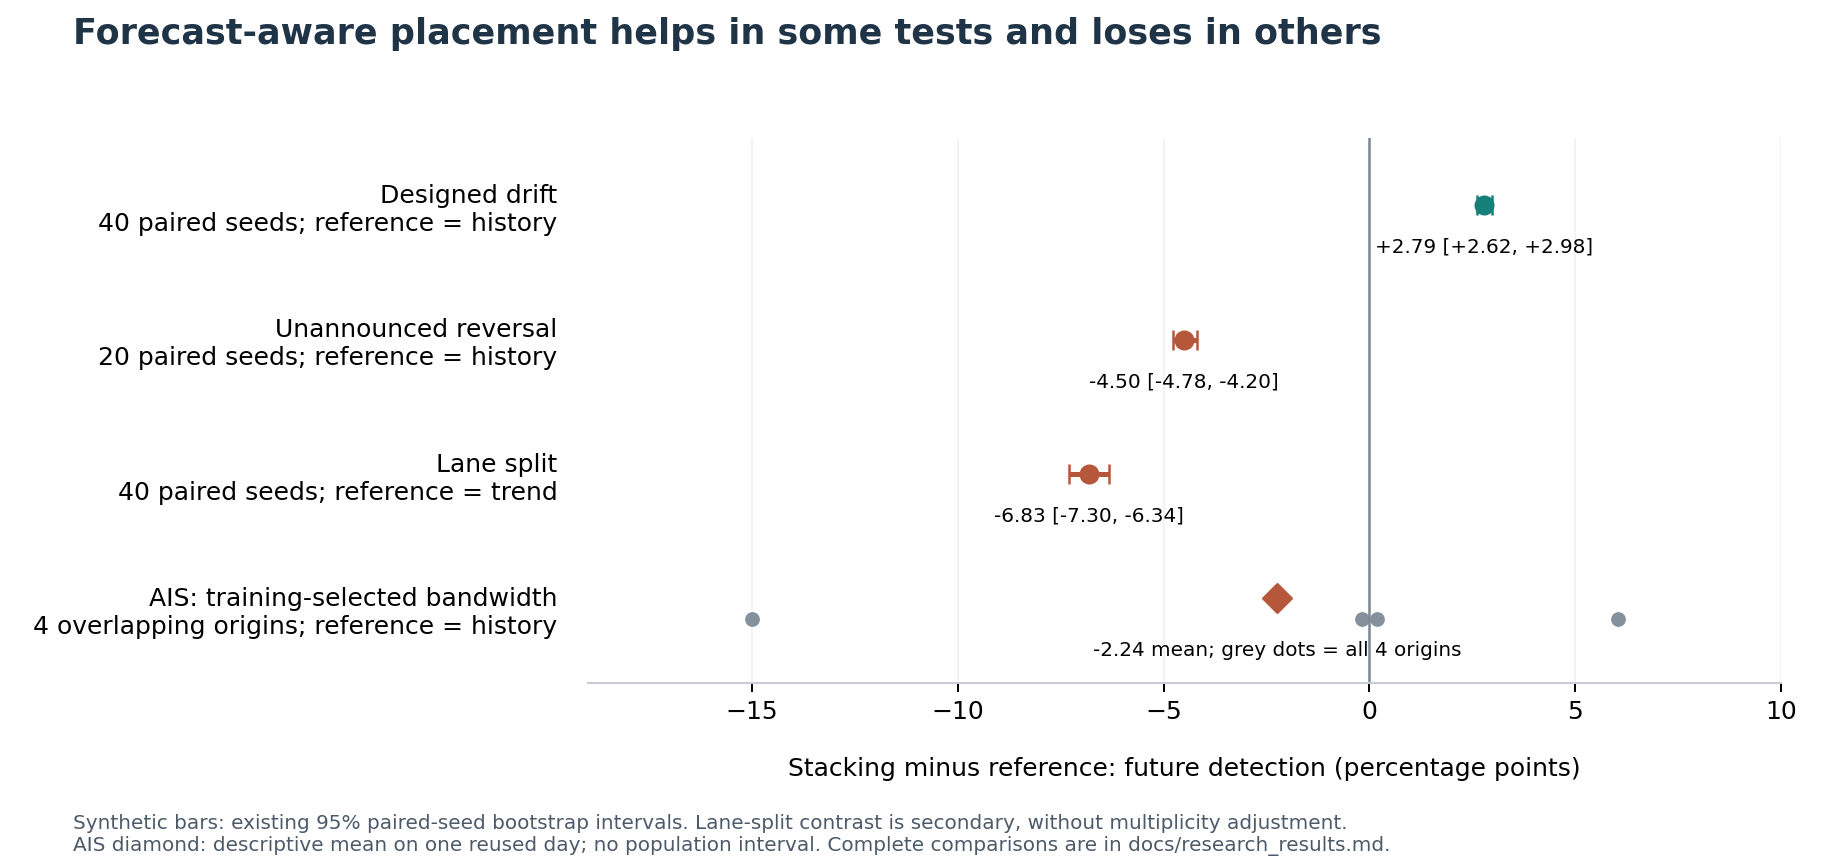
\includegraphics[width=\linewidth]{research_overview.png}
\caption{Successes and failures with each reference named. Synthetic
intervals use the existing paired-seed bootstrap; the lane-split component
contrast is secondary and has no multiplicity adjustment. AIS points show
all four overlapping origins and their descriptive mean, not a population
interval. Outcomes are modelled detection probabilities.}
\end{figure}

\section{Question and relationship to the base framework}
Kim et al.~\cite{kim2025barrier} formulate two-dimensional barrier coverage
for stochastic straight-line trajectories, using a line-space
representation, a log-Gaussian Cox line process and greedy placement with
numerical refinement. Their earlier work~\cite{kim2023toward} establishes
the uncertain-intensity void-probability perspective. We ask how a network
placed before a future traffic shift performs when it plans on forecasts,
and what a declared intensity-ambiguity set can guarantee.

The implementation adds chronological forecast comparison, distinct
intensity-stacking and pseudo-BMA baselines, a tail-risk comparison, a
finite-grid TV ambiguity experiment and a reproducible evaluation. The
representation, LGCP family, submodular approximation principle, stacking,
CVaR and robust observation-selection tools are established methods
\cite{nemhauser1978,yao2018stacking,rockafellar2000,krause2008robust}.
This report focuses on their integration, evaluation and failure modes for shifted line traffic.

\Needspace{9\baselineskip}
\section{Model and numerical representation}
A line is represented by $(\alpha,p)$ through
\[
x\cos\alpha+y\sin\alpha=p,\qquad \alpha\in[0,\pi),\quad p\in\R.
\]
For $y=mx+b$, $\alpha=\pi/2+\arctan m$ and
$p=b/\sqrt{1+m^2}$. The identification
$(\alpha,p)\sim(\alpha+\pi,-p)$ must be respected at the representation
seam. The perpendicular distance from sensor $s=(x_s,y_s)$ to a line is
\[
d_s=|x_s\cos\alpha+y_s\sin\alpha-p|.
\]
With conditionally independent sensor detections,
$q_S(\ell)=\prod_{s\in S}(1-P_D(d_s(\ell)))$. Independent Poisson thinning
gives, for fixed line intensity $\lambda$,
\begin{equation}
L(S;\lambda)=\int\lambda q_S,\qquad
P(\text{no missed trajectory})=e^{-L(S;\lambda)}.
\end{equation}
Expected detection fraction is $1-L/\int\lambda$; it is not the probability
of detecting every trajectory in an epoch.

The grid spans the full angle range and a signed-offset range covering
the deployment window. Gaussian kernels are integrated over cells, with
seam images. Sensor detection is evaluated at cell centres and cells are
masked using their central line. Thus numerical detection scores are
quadrature approximations. Synthetic plans are evaluated on a three-times
finer grid along each axis.

Historical intensities are estimated by KDE or a lattice LGCP with
Poisson cell counts and precision $Q=\tau(\kappa^2I+L_g)^2$, where $L_g$ is
a graph Laplacian including the seam. The posterior uses a Laplace
approximation with plug-in hyperparameters. This is a lattice,
SPDE-inspired model~\cite{lindgren2011}, not R-INLA or a reproduction of
the base paper's inference pipeline~\cite{rue2009inla}.

\section{Forecasting and chronological combination}
Epochs $0,\ldots,T-1$ are observed and the target is $T-1+h$. Forecasts
include pooled history, the two most recent epochs, centroid drift,
uncertainty-expanded drift and a clipped cellwise log-linear trend.
Drift coordinates are lifted continuously across the representation seam.
Gaussian shift uncertainty widens a Gaussian kernel by adding covariance;
its estimated covariance and small-sample inflation are modelling choices,
not a calibrated posterior for every traffic regime.

For held-out target $u$, training uses only the prefix of length $u-h+1$.
Bandwidth is refitted on that prefix. For component intensities
$\lambda_{k,u}$, intensity stacking selects simplex weights to maximise
\begin{equation}
\sum_u\left[\sum_{\ell\in D_u}\log\left(\sum_k w_k\lambda_{k,u}(\ell)\right)
-\sum_k w_k\int\lambda_{k,u}\right].
\end{equation}
The negative objective is convex in $w$, and is optimised with an analytic
gradient and a common numerical log floor. Final component forecasts are
then fitted to all available history. A Poisson process at the combined
intensity differs from a mixture of full predictive point-process laws.
The stacking literature~\cite{yao2018stacking} motivates combination but
is not invoked to assert an equivalence between those models.

The separate pseudo-BMA baseline uses the softmax of each component's
held-out total score. Neither method's weights are asserted to be Bayesian
posterior model probabilities. A fixed equal-weight mixture retains the
original prototype's idea as another baseline.

\section{Objectives and the limits of their guarantees}
For predictive intensity $\Lambda$, the expected objective needs only its
mean: $\E L(S;\Lambda)=L(S;\E\Lambda)$. This identity provides a sufficient
posterior-mean interpretation when a posterior is specified; it does not
imply that posterior weights are necessary for a particular optimal plan.

We compare expected misses, predictive void loss
$-\log\E e^{-L}$ and upper-tail CVaR. Predictive void loss is a soft minimum
of sampled losses, emphasising favourable futures; it is not a worst-case
penalty. For stacking, samples select one forecast component at a time
using its fitted weight. This defines a probability law, but neither a
posterior interpretation of the weights nor calibration is established.
Favourable component draws can dominate the soft minimum.
For equally weighted sampled losses $l_i$, CVaR at level $\beta$ is
\[
\min_\eta\left[\eta+\frac{1}{n(1-\beta)}\sum_i(l_i-\eta)_+\right].
\]
The implementation includes fractional mass at the tail boundary. For
losses $0,1,\ldots,31$ at level $0.9$, the answer is $29.875$; rounding up
to four equally weighted observations would instead give $29.5$.

The predictive intensity samples for void and CVaR have not been validated
for calibration. These comparisons are sensitivity analyses of the supplied
law, not decisions under established uncertainty. Both stacking and
pseudo-BMA use component selection. The weights are valid sampling
probabilities, but neither their posterior interpretation nor uncertainty
calibration is established. The fixed mixture carries no samples and uses
only its mean field. Weighted-sum sampling would be a different modelling
proposal; matching the mean would not by itself validate that proposal.

For expected detected mass, the standard greedy guarantee is $1-1/e$
relative to the best subset of the finite candidate set
\cite{nemhauser1978}. It does not carry over to missed mass, continuous
placement or nonlinear risk objectives. Continuous refinement and
nonlinear-objective greedy search remain heuristics.

\subsection{A sensitivity diagnostic}
Let $\hat S$ be a plan made using $\hat\lambda$ and $S_{\rm ref}$ the
same heuristic given true future intensity $\lambda$. Define
$R=L(\hat S;\lambda)-L(S_{\rm ref};\lambda)$ and
$\delta=L(\hat S;\hat\lambda)-L(S_{\rm ref};\hat\lambda)$. Then
\begin{equation}
R\le\max(\delta,0)+\int|\lambda-\hat\lambda|
\max(1-q_{\hat S},1-q_{S_{\rm ref}})
\le\max(\delta,0)+\|\lambda-\hat\lambda\|_1.
\end{equation}
This follows by linearity and $|a-b|\le\max(1-a,1-b)\le1$ for
$a,b\in[0,1]$. It is an elementary sensitivity inequality. The reference
is not a certified optimum, $\delta$ is a measured comparison term and
neither truth nor the reference is observable at deployment. Simulation
checks verify numerical consistency, not an independent generalisation
guarantee. Equal-total Poisson score and Pinsker's inequality motivate
log-score validation, but do not guarantee lower regret on every future.

\subsection{Finite-grid TV ambiguity}
For nominal active-cell masses $m\ge0$, total $N=\sum_i m_i$ and
$\epsilon\in[0,1]$, define
\[
\mathcal M_\epsilon(m)=\{z\ge0:\mathbf1^Tz=N,\ \tfrac12\|z-m\|_1\le\epsilon N\},
\qquad \rho_\epsilon(S;m)=\max_{z\in\mathcal M_\epsilon(m)}z^Tq_S.
\]
\begin{proposition}[Exact finite-grid inner adversary]
A maximiser transfers up to $\epsilon N$ mass from cells in increasing
order of miss probability to a maximum-miss cell, stopping once remaining
donors have that maximum miss probability. Moreover,
\[
m^Tq_S\le\rho_\epsilon(S;m)\le
\min\{Nq_{\max},m^Tq_S+\epsilon N(q_{\max}-q_{\min})\}.
\]
\end{proposition}
\begin{proof}
Every feasible change transfers at most $\epsilon N$ mass. A unit of
recipient mass contributes most at $q_{\max}$. Given that recipient,
removing mass from a higher-loss donor while a lower-loss donor has mass
cannot improve the objective, so an exchange argument orders donors.
No positive gain remains after nonmaximum donors are exhausted.
\end{proof}
If normalised grid truth $p$ satisfies
$\tfrac12\|p-m/N\|_1\le\epsilon$, then its expected detection is at least
$1-\rho_\epsilon/N$. This certificate is conditional on the declared grid
and ambiguity set. The inner solution is checked against a separate LP;
the outer sensor problem uses greedy initialisation and one-sensor
exchanges, with no global approximation claim. Choosing a radius does not
establish that future traffic lies inside the ball.

\section{Evaluation and findings}
\subsection{Main synthetic comparison}
Four designed regimes use eight history epochs, four Gaussian sensors,
a two-epoch horizon, 40 seeds and known future intensity. Comparisons are
paired by seed, with percentile bootstrap intervals. Candidate spacing is
one unit and the deployment window is $20\times10$ units. The configs and
raw outputs are the authoritative experimental specification.

\begin{table}[ht]
\centering\small
\caption{Gap to the true-intensity heuristic reference in percentage
points, lower is better. Intervals are paired-study summaries over 40
seeds. The reference is not a global optimum.}
\resizebox{\linewidth}{!}{\begin{tabular}{lcccc}
\toprule
Planner & Stationary & Drift & Lane shift & Emergence\\\midrule
Historical, KDE & 0.24 {\scriptsize[0.19, 0.31]} & 2.98 {\scriptsize[2.82, 3.17]} & 1.40 {\scriptsize[1.37, 1.43]} & 1.98 {\scriptsize[1.44, 2.52]} \\
Historical, LGCP & 0.23 {\scriptsize[0.18, 0.29]} & 3.45 {\scriptsize[3.23, 3.69]} & 1.45 {\scriptsize[1.42, 1.48]} & 2.22 {\scriptsize[1.70, 2.73]} \\
Recent epochs only & 0.30 {\scriptsize[0.25, 0.36]} & 1.98 {\scriptsize[1.75, 2.23]} & 0.29 {\scriptsize[0.24, 0.34]} & 0.33 {\scriptsize[0.20, 0.48]} \\
Drift extrapolation & 0.26 {\scriptsize[0.21, 0.31]} & \textbf{0.18 {\scriptsize[0.15, 0.21]}} & 1.53 {\scriptsize[1.46, 1.59]} & 1.87 {\scriptsize[1.51, 2.26]} \\
Drift + uncertainty & 0.37 {\scriptsize[0.31, 0.44]} & 0.19 {\scriptsize[0.16, 0.23]} & 1.92 {\scriptsize[1.85, 1.98]} & 2.39 {\scriptsize[2.06, 2.69]} \\
Log-linear trend & 0.71 {\scriptsize[0.63, 0.79]} & 2.22 {\scriptsize[1.99, 2.47]} & 0.30 {\scriptsize[0.25, 0.36]} & \textbf{0.08 {\scriptsize[0.02, 0.14]}} \\
$\lambda_E$ with fixed weights (v0.1 idea) & 0.29 {\scriptsize[0.23, 0.34]} & 0.85 {\scriptsize[0.81, 0.90]} & 1.47 {\scriptsize[1.42, 1.51]} & 2.43 {\scriptsize[2.05, 2.79]} \\
Pseudo-BMA (score-weighted baseline) & 0.22 {\scriptsize[0.17, 0.28]} & 0.19 {\scriptsize[0.16, 0.23]} & 0.30 {\scriptsize[0.25, 0.36]} & 0.44 {\scriptsize[0.23, 0.70]} \\
Stacked $\lambda_E$ (ours) & 0.23 {\scriptsize[0.18, 0.28]} & 0.20 {\scriptsize[0.16, 0.24]} & \textbf{0.23 {\scriptsize[0.19, 0.29]}} & 0.29 {\scriptsize[0.15, 0.46]} \\
Stacked $\lambda_E$, expected void objective & 0.25 {\scriptsize[0.19, 0.31]} & 3.67 {\scriptsize[2.90, 4.44]} & 0.24 {\scriptsize[0.19, 0.29]} & 0.32 {\scriptsize[0.22, 0.42]} \\
Stacked $\lambda_E$, CVaR objective & 0.31 {\scriptsize[0.24, 0.38]} & 0.36 {\scriptsize[0.29, 0.45]} & 0.61 {\scriptsize[0.47, 0.77]} & 1.05 {\scriptsize[0.79, 1.32]} \\
Drift + uncertainty, expected void objective & \textbf{0.22 {\scriptsize[0.19, 0.24]}} & 0.19 {\scriptsize[0.16, 0.23]} & 1.84 {\scriptsize[1.70, 2.01]} & 1.91 {\scriptsize[1.60, 2.22]} \\
Drift + uncertainty, CVaR objective & 0.97 {\scriptsize[0.84, 1.12]} & 0.25 {\scriptsize[0.21, 0.30]} & 3.43 {\scriptsize[3.21, 3.67]} & 1.60 {\scriptsize[1.37, 1.82]} \\
Log-linear trend, CVaR objective & 1.65 {\scriptsize[1.42, 1.88]} & 1.62 {\scriptsize[1.40, 1.88]} & 0.69 {\scriptsize[0.56, 0.83]} & 0.60 {\scriptsize[0.42, 0.82]} \\
Evenly spaced fence & 12.2 & 17.1 & 27.6 & 25.2 \\
Random & 29.1 & 41.8 & 28.8 & 30.6 \\
\bottomrule

\end{tabular}}
\end{table}

Intensity stacking changes expected misses relative to pooled history by
\missRedStat\% [\missRedLoStat, \missRedHiStat] in stationary traffic,
\missRedDrift\% [\missRedLoDrift, \missRedHiDrift] under drift,
\missRedShift\% [\missRedLoShift, \missRedHiShift] under lane shift and
\missRedEmerg\% [\missRedLoEmerg, \missRedHiEmerg] under emergence.
These are relative reductions, not percentage-point detection gains.
The successful regimes closely match candidates: constant-velocity drift
matches the drift model, logit-linear lane shares resemble cellwise
log-linear trend, and stationarity matches pooled history. These gains
show selection of a well-specified candidate, not generalisation to shifts
outside every candidate family. The reversal is outside those families:
history detects \reversalHistory\% versus stacking's \reversalStacked\%.
This is an experimental-design limitation affecting the headline results,
not an implementation bug. The generators do not establish how frequently
these regimes arise operationally.

Expected-void planning on the stacked forecast is a separate failure under
 drift: its reference gap is \voidDriftGap{} [\voidDriftGapLo,
\voidDriftGapHi] percentage points, with \voidDriftOverOne{} of
\voidDriftSeeds{} seeds above one point. Its detection difference from
history is \voidDriftHistory{} [\voidDriftHistoryLo,
\voidDriftHistoryHi] points. The interval includes zero, so this is a lower
mean in these runs, not an established loss across seeds. The gap's
correlation with non-drift component weight is \voidDriftCorr. The
component sampler and the soft minimum's preference for favourable draws
are relevant mechanisms; correlation alone does not establish causation.

\begin{figure}[ht]
\centering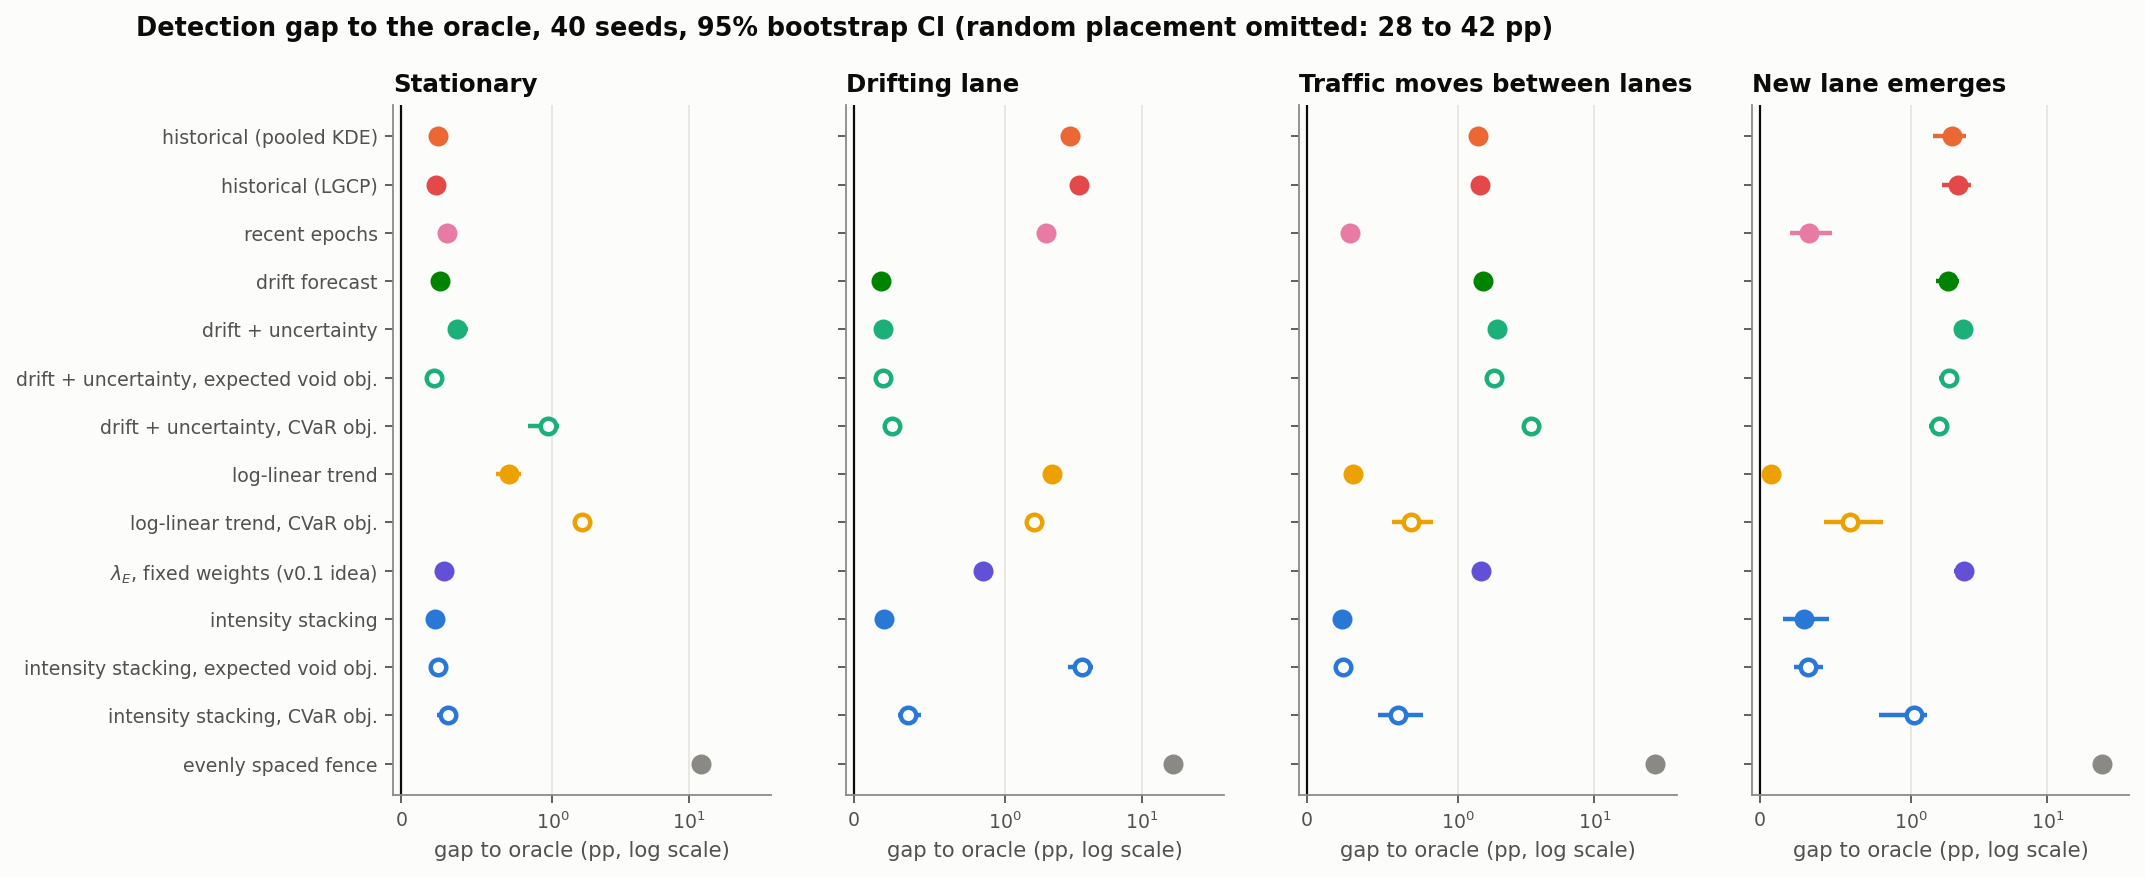
\includegraphics[width=\linewidth]{scenario_suite.png}
\caption{Main synthetic comparison, evaluated on the true future. The
oracle label denotes the true-intensity heuristic reference.}
\end{figure}
\FloatBarrier

\subsection{Stress tests and the cost of an unstructured ambiguity set}
The robustness study uses 20 paired seeds in six scenarios, common
finite-grid candidates, and radii $0$, $0.05$ and $0.15$. All planners use
one-sensor exchange refinement. Unlike the main experiment, no continuous
refinement is used, so absolute rates should not be compared across the
two studies as if only the risk objective had changed.

When drift reverses just after training, historical placement detects
\reversalHistory\% of future trajectories while intensity stacking detects
\reversalStacked\%. The turn is not revealed to forecasters. This is an
explicit counterexample to a universal benefit from extrapolation.

\begin{figure}[ht]
\centering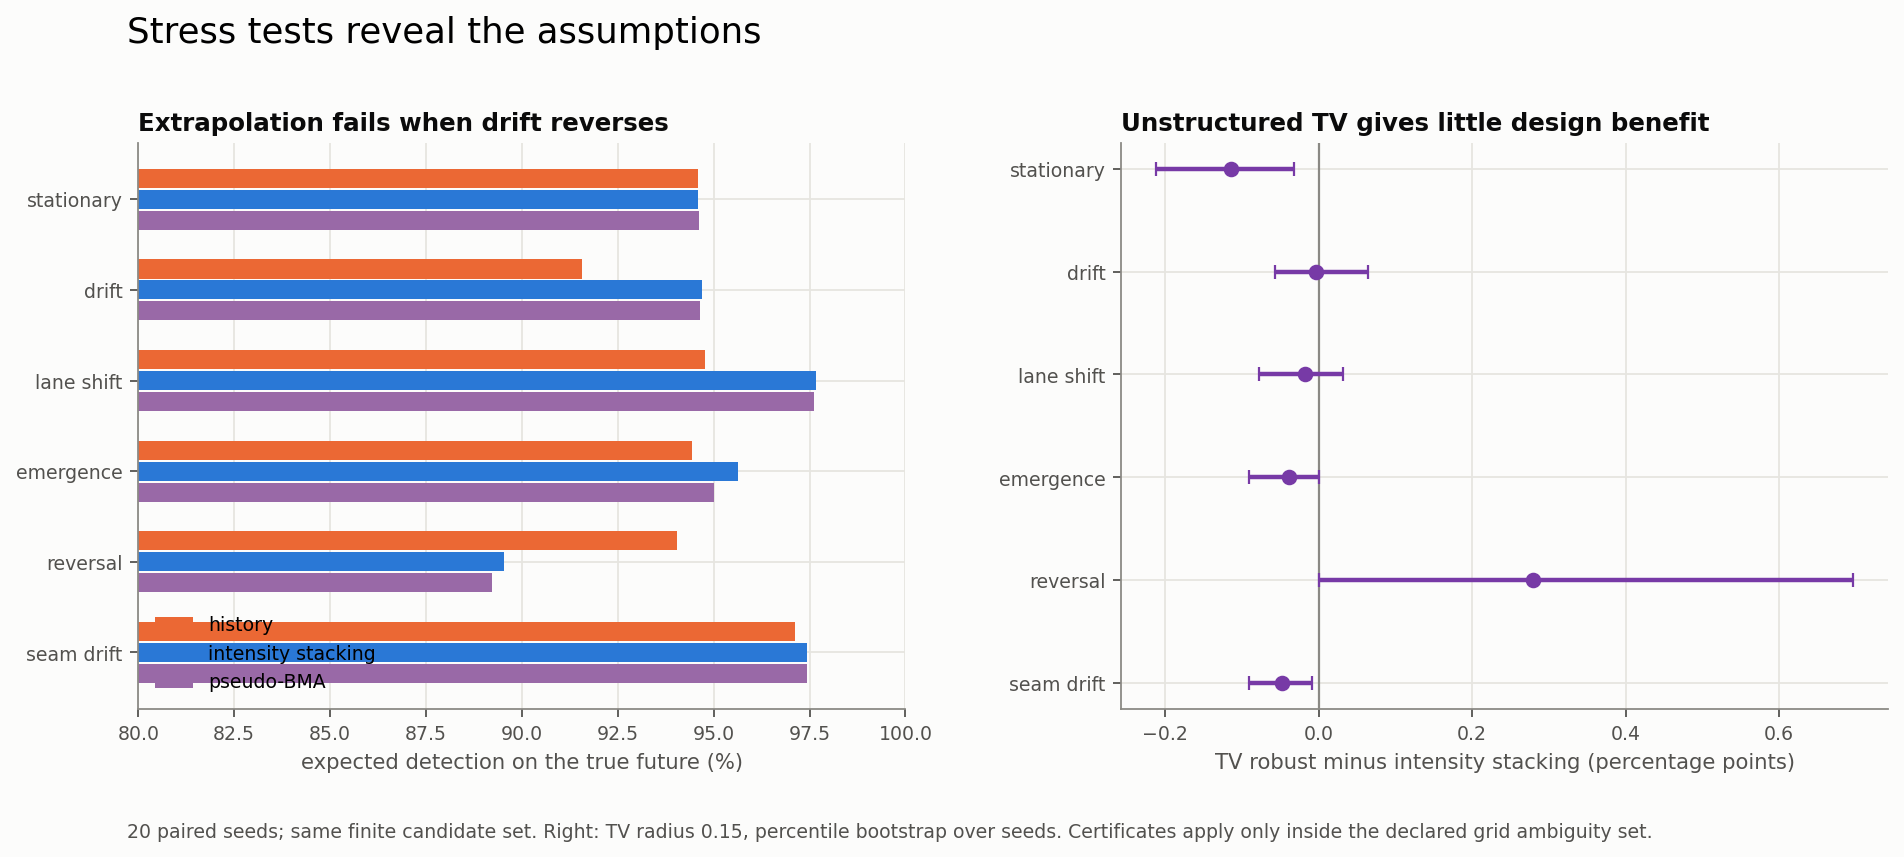
\includegraphics[width=\linewidth]{forecast_failure.png}
\caption{Stress tests expose both forecast failure and the limited design
leverage of unrestricted TV ambiguity. Right: change in future detection,
TV radius $0.15$, with paired-seed bootstrap intervals.}
\end{figure}

\begin{table}[ht]
\centering\small
\caption{TV robust placement minus intensity stacking, radius $0.15$.
Future change uses finer-grid truth; worst-case change uses the planning
grid. The final column is the fraction of simulated truths inside the
stated ambiguity ball, not an estimated operational coverage guarantee.}
\begin{tabular}{lrrr}
\toprule
Scenario & Future change (pp) & Worst-case change (pp) & Inside ball\\\midrule
Stationary & -0.114 & +0.041 & 95\% \\
Drift & -0.004 & +0.052 & 95\% \\
Lane shift & -0.018 & +0.016 & 0\% \\
Emergence & -0.039 & +0.003 & 0\% \\
Reversal & +0.279 & +0.101 & 0\% \\
Seam drift & -0.047 & +0.006 & 95\% \\
\bottomrule

\end{tabular}
\end{table}

The TV penalty can change little across plausible plans: many grids have
almost-uncovered recipient cells and well-covered donor mass, making the
adversarial surcharge close to $\epsilon N$ across different placements.
The experiment therefore does not establish a substantial TV design gain.
Across all saved strategies, nominal minus worst-case detection spans
\tvPenaltyFiveMin{} to \tvPenaltyFiveMax{} points at radius $0.05$ and
\tvPenaltyFifteenMin{} to \tvPenaltyFifteenMax{} points at $0.15$.
At radius $0.05$, no scenario-strategy group has truth coverage above
\tvSmallCoverageMax\%. At $0.15$, stacked-forecast coverage is
\tvCoverageStationary\% for stationary, \tvCoverageDrift\% for drift and
\tvCoverageSeamDrift\% for seam traffic; it is \tvCoverageLaneShift\%
for lane shift, \tvCoverageEmergence\% for emergence and
\tvCoverageReversal\% for reversal. These are grid-based simulated
coverage fractions, not a calibration guarantee.
A few small negative worst-case differences also expose the limits of the
heuristic outer search. Geometry-constrained ambiguity and calibrated radii
are useful next research questions, not completed results here.
The maximum absolute coarse/fine detection difference in this study is
\robustGridErrorMax{} percentage points, reinforcing why certificate and
fine-grid score must be kept distinct.
\FloatBarrier

\subsection{AIS demonstration}
A checksummed public sample contains \aisReports{} AIS reports near
Gothenburg on 5 July 2017, yielding \aisLines{} straight pieces after
filtering. Reports are split at time gaps, window exits, low-speed reports
and three-hour epoch boundaries before line fitting. Four rolling origins
plan on earlier epochs and score the next epoch's observed pieces.

Historical KDE has mean expected detection \aisPooled\% and intensity
stacking \aisStacked\%. At the default bandwidth, historical LGCP leads the KDE planners by
\aisBandwidthGapMin{} to \aisBandwidthGapMax{} percentage points.
A post hoc multiplier of $0.25$ gives historical KDE \aisFinePooled\%,
stacking \aisFineStacked\% and LGCP \aisFineLgcp\%; recent epochs remain
\aisFineRecentGap{} points behind LGCP. Only final component fits are rescaled
in this probe; stacking weights come from default-bandwidth backtests.
Historical KDE approaches LGCP at finer resolution, but this does not
establish equivalence. Rescaling every nested prefix in C4 gives stacking
\aisNestedStacked\% on this reused day (Appendix~A).
This probe was computed after viewing the test epochs and is sensitivity
evidence only. No scale is adopted. It does not settle history versus forecast. The one-day sample is too small for a broad
real-world claim. Table~\ref{tab:ais-origins} reports every origin and
paired differences from historical KDE rather than bootstrap intervals.
Origins overlap in training history and do not support population-level
significance claims. Metrics use modelled detection per straight piece,
not actual sensor measurements or necessarily distinct ships.

\begin{table}[ht]
\centering\small
\caption{AIS expected detection (\%) at each origin, with the paired
change from historical KDE in brackets (percentage points). These are
individual test-origin results, not confidence intervals.}
\label{tab:ais-origins}
\begin{tabular}{lrrrr}
\toprule
Planner & Origin 4 & Origin 5 & Origin 6 & Origin 7 \\\midrule
Historical KDE & 81.3 [+0.0] & 79.2 [+0.0] & 69.6 [+0.0] & 76.3 [+0.0] \\
Recent epochs & 79.0 [-2.3] & 78.0 [-1.2] & 79.9 [+10.3] & 73.8 [-2.5] \\
Historical LGCP & 87.6 [+6.3] & 85.1 [+5.9] & 82.8 [+13.2] & 85.3 [+9.0] \\
Intensity stacking & 79.0 [-2.3] & 78.5 [-0.8] & 78.4 [+8.8] & 74.9 [-1.4] \\
Pseudo-BMA & 79.1 [-2.2] & 79.2 [-0.0] & 69.6 [+0.0] & 76.3 [-0.0] \\
Hindsight heuristic & 84.6 [+3.3] & 84.6 [+5.4] & 87.3 [+17.7] & 83.4 [+7.1] \\
\bottomrule

\end{tabular}
\end{table}

\begin{figure}[ht]
\centering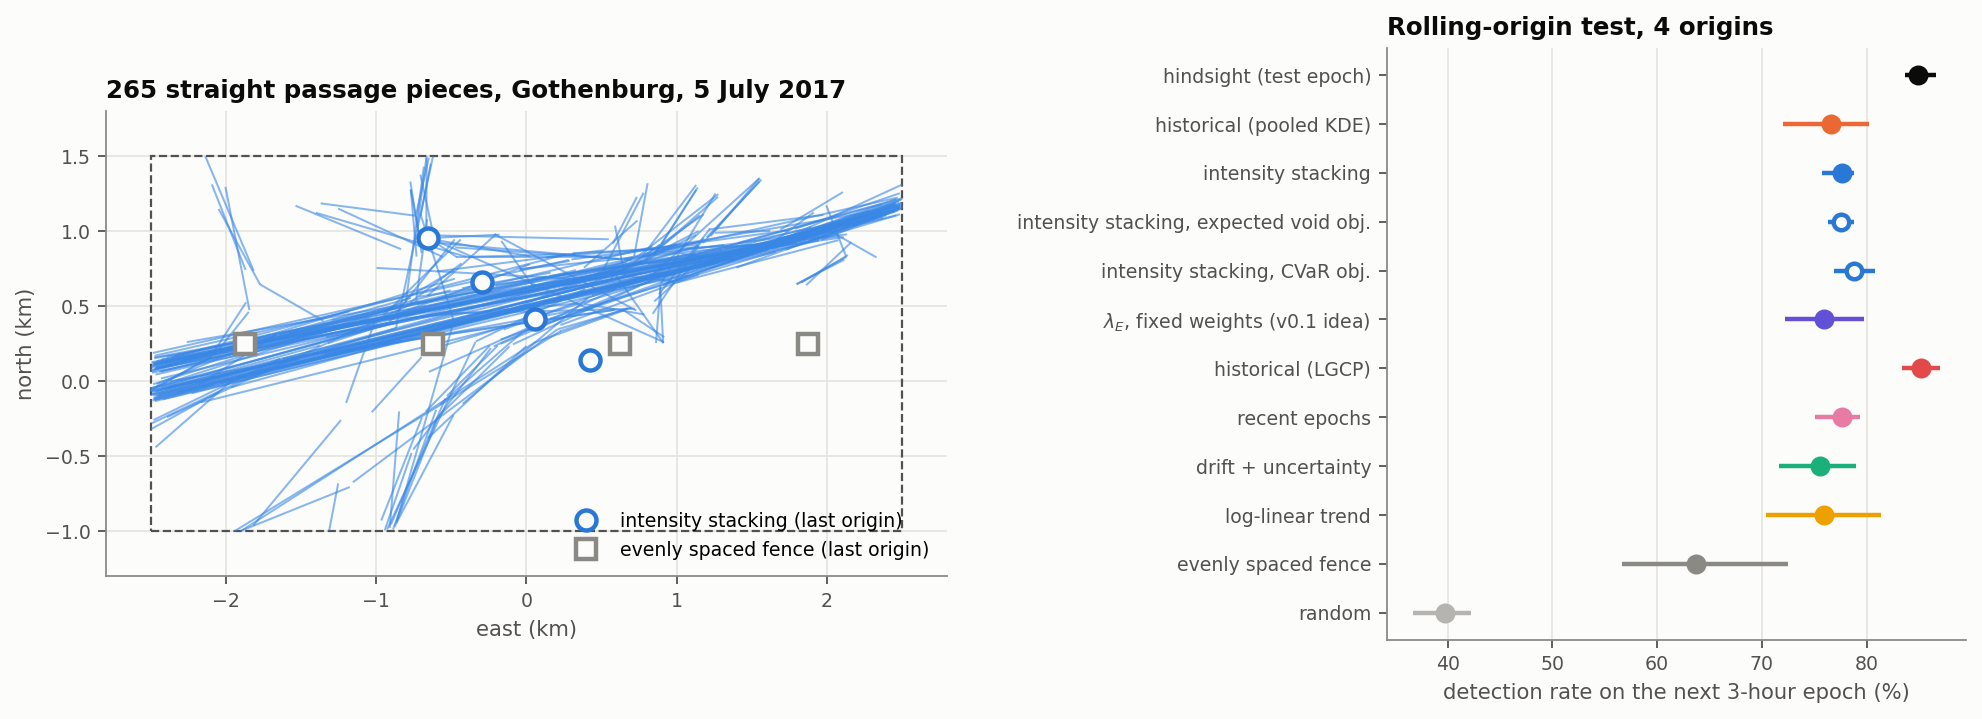
\includegraphics[width=0.90\linewidth]{ais_case_study.png}
\caption{AIS location and descriptive mean summaries. The bars in this
retained visualisation resample the same overlapping origins and are not
population-level confidence statements; use Table~\ref{tab:ais-origins}
for the individual results. Hindsight fits the test epoch but uses a local
heuristic; it is not a strict upper bound.}
\end{figure}
\FloatBarrier

\section{Verification, reproducibility and remaining limits}
Tests compare geometry with independent formulas, analytic gradients with
finite differences, Poisson thinning with simulated detections, greedy
selection with enumeration, fractional CVaR with an epigraph LP and the TV
adversary with a separate LP. Regression fixtures enforce chronological
bandwidth fitting, seam behaviour and AIS epoch boundaries. A parity test
compares the Python legacy port with the unchanged MATLAB script through
GNU Octave when that dependency is available.

Each result set records a source SHA-256, configuration, dependency
versions and Git revision. The artifact verifier recomputes synthetic
summaries, checks run uniqueness and tests every in-scope TV certificate.
A Python 3.12 dependency snapshot, VS Code workspace, task definitions,
learning notebook and reproduction command are supplied. Hosted CI status
must be distinguished from locally completed checks; the validation record
in the repository states exactly what ran.

The model assumes straight trajectories, conditionally independent
isotropic sensors and distance-only detection. It omits propagation,
bathymetry, installation constraints, correlated detection and physical
calibration. Synthetic traffic is designed and AIS evidence is limited.

\Needspace{8\baselineskip}
A useful next evaluation would hold out multiple days and sites, include
known route changes, calibrate uncertainty before scoring and compare
strong domain-specific placement methods. The present result is an
auditable study of when forecast-aware placement helps or fails, and why
unstructured TV ambiguity adds little design benefit in these examples.
Operational deployment remains outside the evidence. Appendix~A includes
the locally frozen extension studies: gains over pooled history do not
establish superiority to individual components, and the component losses
and calibration-prefix limitations are shown explicitly.

\bibliographystyle{plainnat}
\bibliography{refs}
\clearpage
\appendix
\section{Locally frozen extension studies}

Protocol and candidate commits precede the outcomes in the preserved local history; no external preregistration timestamp exists. All original study summaries are unchanged relative to the corrected pre-extension checkpoint. New methods remain experimental; no sampler or AIS policy replaces a default.

\Needspace{12\baselineskip}
\paragraph{Shifts outside the candidate families (40 paired seeds)}
\begin{center}\small\begin{tabular}{lll}
\toprule
Regime & Stacked minus history, pp [95\% CI] & Positive seeds\\\midrule
accelerating & +10.74 [+10.25, +11.27] & 40/40\\
lane\_split & +1.00 [+0.63, +1.42] & 36/40\\
random\_switch & +2.57 [+1.80, +3.42] & 32/40\\
random\_walk & +1.14 [+0.36, +2.07] & 26/40\\
rotating\_quadratic & +3.77 [+3.47, +4.10] & 40/40\\
\bottomrule\end{tabular}\end{center}

Intervals resample paired seeds. These are specified synthetic generators, not operational traffic.

\Needspace{12\baselineskip}
\paragraph{Secondary component comparisons}
\begin{center}\small\begin{tabular}{lll}
\toprule
Regime & Component & Stacked minus component, pp [95\% CI]\\\midrule
accelerating & drift\_u & -0.15 [-0.21, -0.09]\\
accelerating & recent & +4.94 [+4.44, +5.52]\\
accelerating & trend & +3.88 [+3.46, +4.33]\\
lane\_split & drift\_u & +0.83 [+0.46, +1.24]\\
lane\_split & recent & -3.77 [-4.19, -3.36]\\
lane\_split & trend & -6.83 [-7.30, -6.34]\\
random\_switch & drift\_u & -0.32 [-1.27, +0.57]\\
random\_switch & recent & -1.33 [-2.18, -0.54]\\
random\_switch & trend & -1.82 [-3.12, -0.62]\\
random\_walk & drift\_u & -0.30 [-1.11, +0.41]\\
random\_walk & recent & -0.49 [-1.04, +0.01]\\
random\_walk & trend & -0.38 [-1.15, +0.29]\\
rotating\_quadratic & drift\_u & -0.01 [-0.01, -0.00]\\
rotating\_quadratic & recent & +3.96 [+3.11, +4.98]\\
rotating\_quadratic & trend & +5.36 [+4.51, +6.33]\\
\bottomrule\end{tabular}\end{center}

These descriptive comparisons were added after the audit. The primary contrast remains stacked minus pooled; complete comparisons with every strategy are in the generated holdout component table. Intervals are not adjusted for multiple comparisons.

\clearpage

\Needspace{12\baselineskip}
\paragraph{Sampler diagnostics on the same expected-loss plans}
\begin{center}\small\begin{tabular}{lllll}
\toprule
Regime & Sampler & Rank & Coverage & Mismatch\\\midrule
accelerating & component & 0.714 & 62.5\% & 0.038\\
accelerating & residual\_candidate & 0.654 & 97.5\% & 0.126\\
accelerating & weighted\_candidate & 0.757 & 42.5\% & 0.041\\
lane\_split & component & 1.000 & 0.0\% & 0.015\\
lane\_split & residual\_candidate & 1.000 & 0.0\% & 0.041\\
lane\_split & weighted\_candidate & 1.000 & 0.0\% & 0.008\\
random\_switch & component & 0.720 & 50.0\% & 0.046\\
random\_switch & residual\_candidate & 0.770 & 42.5\% & 0.072\\
random\_switch & weighted\_candidate & 0.701 & 22.5\% & 0.031\\
random\_walk & component & 0.312 & 10.0\% & 0.020\\
random\_walk & residual\_candidate & 0.380 & 42.5\% & 0.055\\
random\_walk & weighted\_candidate & 0.293 & 5.0\% & 0.014\\
rotating\_quadratic & component & 0.916 & 32.5\% & 0.039\\
rotating\_quadratic & residual\_candidate & 0.662 & 100.0\% & 0.190\\
rotating\_quadratic & weighted\_candidate & 0.922 & 32.5\% & 0.043\\
\bottomrule\end{tabular}\end{center}

The gate requires every regime to have at least 80\% coverage, mean rank in $[.35,.65]$ and mean relative sample-mean mismatch at most $.10$. Eligibility for further study: weighted\_candidate fails; residual\_candidate fails. No sampler is adopted. These are latent-loss ensemble diagnostics, not realized-count PIT or validation of the full point-process law. Fixed Monte Carlo streams are reused across history seeds: these are conditional diagnostics with common random numbers, not independent sampler-noise realizations.

\clearpage

\Needspace{12\baselineskip}
\paragraph{Training-only AIS bandwidth selection}
\begin{center}\small\begin{tabular}{lllll}
\toprule
Origin & Method & Scale & Detection & Paired change, pp\\\midrule
4 & pooled & 0.25 & 87.35\% & +6.04\\
4 & recent & 0.25 & 88.22\% & +6.91\\
4 & stacked & 0.25 & 87.53\% & +6.23\\
5 & pooled & 0.25 & 84.53\% & +5.30\\
5 & recent & 0.25 & 83.65\% & +4.42\\
5 & stacked & 0.25 & 84.36\% & +5.13\\
6 & pooled & 0.25 & 75.02\% & +5.44\\
6 & recent & 0.25 & 80.54\% & +10.95\\
6 & stacked & 0.25 & 81.07\% & +11.48\\
7 & pooled & 0.25 & 92.24\% & +15.96\\
7 & recent & 0.25 & 78.80\% & +2.53\\
7 & stacked & 0.25 & 77.23\% & +0.96\\
\bottomrule\end{tabular}\end{center}

Changes use the default historical KDE reference. Selection uses targets strictly before each test origin. The previously viewed one-day sample is reused: this is exploratory reanalysis, with no population significance claim.

12/12 choices select 0.25, the lower edge of the frozen grid; the grid does not bracket an interior optimum. It is not extended on this reused day. Stacking exceeds pooled history at 2/4 origins; its largest deficit, at origin 7, drives the mean comparison.

\Needspace{12\baselineskip}
\paragraph{AIS policy ablations (mean over four origins)}
\begin{center}\small\begin{tabular}{llll}
\toprule
Method & Policy & Detection & Paired change, pp\\\midrule
pseudo\_bma & both & 76.60\% & +0.00\\
pseudo\_bma & minimum\_origins & 76.60\% & -0.00\\
pseudo\_bma & original & 76.04\% & -0.56\\
pseudo\_bma & relative\_floor & 76.04\% & -0.56\\
stacked & both & 78.44\% & +1.84\\
stacked & minimum\_origins & 78.44\% & +1.84\\
stacked & original & 77.66\% & +1.06\\
stacked & relative\_floor & 77.66\% & +1.06\\
\bottomrule\end{tabular}\end{center}

Origin-level weights, solver status and all individual detections are retained in the raw CSV and the generated AIS policy table. Minimum-origin and relative-floor rules are ablations only; the original policy remains the default.

\clearpage

\Needspace{12\baselineskip}
\paragraph{Geometry-aware ambiguity (20 paired seeds)}
\begin{center}\small\begin{tabular}{llllll}
\toprule
Regime & Ball & Future gain, pp [95\% CI] & Inside & Changed & WC gain\\\midrule
drift & tv & -0.476 [-0.858, -0.095] & 100\% & 5/20 & +0.045\\
drift & w1 & -10.378 [-12.405, -7.865] & 100\% & 20/20 & +6.548\\
emergence & tv & +0.000 [+0.000, +0.000] (D) & 65\% & 0/20 & +0.000\\
emergence & w1 & -5.274 [-5.738, -4.757] & 50\% & 20/20 & +3.763\\
lane\_shift & tv & -1.085 [-1.640, -0.586] & 100\% & 10/20 & +0.134\\
lane\_shift & w1 & -18.263 [-20.759, -16.684] & 100\% & 20/20 & +10.293\\
reversal & tv & -0.519 [-1.618, +0.428] & 20\% & 3/20 & +0.041\\
reversal & w1 & -16.070 [-16.070, -16.070] (D) & 30\% & 20/20 & +10.735\\
seam\_drift & tv & -2.816 [-3.840, -1.792] & 100\% & 11/20 & +0.129\\
seam\_drift & w1 & -2.114 [-3.423, -1.052] & 100\% & 8/20 & +0.121\\
stationary & tv & +0.000 [+0.000, +0.000] (D) & 100\% & 0/20 & +0.000\\
stationary & w1 & -0.835 [-0.982, -0.688] & 95\% & 17/20 & +0.786\\
\bottomrule\end{tabular}\end{center}

The transport plan lowers mean future detection in 6/6 tested regimes under this fixed calibration rule. This negative result does not isolate geometry as the cause.

The finite-grid transport dual was checked against an independently formulated primal LP on four-cell unit fixtures. Every certificate is conditional on normalized grid truth lying in its ball. Three chronological training errors do not establish nominal coverage. Search is discrete and heuristic; no global placement or operational guarantee is claimed. The Wasserstein construction is established \citep{gao2023wasserstein,esfahani2018wasserstein}; distributionally robust coverage control also predates this study \citep{boskos2023coverage}.

The first calibration target (5) uses four history epochs: stacking has no usable weight-validation backtest and returns pooled history. Thus radii can be driven by an immature pooled forecast rather than the eight-epoch stacked plan. This also affects the first residual-bootstrap factor in C3. These negative results are conditional on the fixed calibration rule; they do not isolate geometry as the cause. The rule and all original outcomes are retained.

\clearpage

\Needspace{12\baselineskip}
\paragraph{Distinct discrete plans across 20 history seeds}
\begin{center}\small\begin{tabular}{llll}
\toprule
Regime & Ball & Nominal & Robust\\\midrule
drift & tv & 2 & 2\\
drift & w1 & 2 & 2\\
emergence & tv & 2 & 2\\
emergence & w1 & 2 & 7\\
lane\_shift & tv & 3 & 2\\
lane\_shift & w1 & 3 & 4\\
reversal & tv & 1 & 3\\
reversal & w1 & 1 & 1\\
seam\_drift & tv & 1 & 2\\
seam\_drift & w1 & 1 & 3\\
stationary & tv & 2 & 2\\
stationary & w1 & 2 & 2\\
\bottomrule\end{tabular}\end{center}

Intervals marked (D) have zero width and are degenerate; they reflect repeated discrete plans, not population precision.

\Needspace{12\baselineskip}
\paragraph{Calibration-rule diagnostic}
\begin{center}\small\begin{tabular}{llll}
\toprule
Regime & Ball & First error sets radius & Median radius/truth distance\\\midrule
drift & tv & 20/20 & 5.02\\
drift & w1 & 20/20 & 6.44\\
emergence & tv & 1/20 & 1.14\\
emergence & w1 & 1/20 & 1.05\\
lane\_shift & tv & 20/20 & 3.98\\
lane\_shift & w1 & 20/20 & 13.16\\
reversal & tv & 20/20 & 0.98\\
reversal & w1 & 20/20 & 0.97\\
seam\_drift & tv & 20/20 & 9.10\\
seam\_drift & w1 & 20/20 & 4.22\\
stationary & tv & 6/20 & 1.85\\
stationary & w1 & 4/20 & 3.01\\
\bottomrule\end{tabular}\end{center}

These truth-distance ratios are retrospective diagnostics and never select a radius. The first calibration prefix returns pooled history because no weight-validation backtest is usable.

\paragraph{Multi-week AIS (C7)} The proposed July 2020 routing-change study remains blocked by archive access. No raw archive, checksum or multi-week result is reported. Settings and the data dependency are recorded in the repository.

\end{document}
